\chapter{Análise de requisitos}

Na análise de requisitos, a primeira atividade consistiu na definição do problema em conjunto com os \textit{stakeholders}, entendidos como as partes interessadas e impactadas pela proposta. Em seguida, foi elaborada uma análise das causas-raízes dos problemas, permitindo compreender como as necessidades dos usuários poderiam ser atendidas pelas funcionalidades da solução.

\section{Definição do problema}

Considerando as dificuldades enfrentadas por muitos usuários no acompanhamento e na interpretação de suas informações financeiras no dia a dia, torna-se possível identificar, por meio do Quadro~\ref{frame:problema}, a definição do problema que fundamenta o EIGAM.

{\small
\begin{longtable}{|l|L{10cm}|}
\caption{Definição do problema}
\label{frame:problema} \\
\continuesmark
\hline
\endfirsthead
\hline
\endhead
\endfoot
\sourcerow{2} \\
\endlastfoot
\textbf{Problema} & Dificuldade em acompanhar, interpretar e utilizar de forma prática as informações financeiras pessoais no dia a dia. \\ \hline
\textbf{Afeta} & Jovens de 18 a 30 anos, como estudantes, estagiários, profissionais em início de carreira e autônomos, que utilizam serviços bancários digitais e desejam maior controle sobre seus gastos, compromissos financeiros e planejamento pessoal. \\ \hline
\textbf{Devido} & À complexidade das informações financeiras, à necessidade de acessar aplicativos ou sistemas específicos para consulta, à baixa integração dessas ferramentas com a rotina do usuário e à dificuldade em transformar dados bancários em orientações simples, úteis e acessíveis para a tomada de decisão. \\ \hline
\textbf{Benefícios} & Com uma solução de assistência financeira inteligente operada pelo WhatsApp e por outros canais de mensageria, integrada ao Open Finance e apoiada por recursos de análise preditiva e interação em linguagem natural, os usuários acompanham suas finanças com mais praticidade, compreendem melhor seus hábitos de consumo, recebem avisos e orientações personalizadas e tomam decisões financeiras de maneira mais consciente, rápida e acessível. \\ \hline
\end{longtable}
}

\section{\textit{Stakeholders}}

A identificação dos \textit{stakeholders} é fundamental para compreender os atores envolvidos no projeto, especialmente aqueles que mantêm interesse direto ou influência sobre a aplicação proposta. Nesse contexto, o Quadro~\ref{frame:stakeholders} apresenta os \textit{stakeholders} relacionados à solução, bem como sua classificação e o grau de influência atribuído a cada um.

\begin{table}[H]
\centering
\caption{\textit{Stakeholders}}
\label{frame:stakeholders}
\begin{tabular}{|l|l|l|}
\hline
\textbf{\textit{Stakeholders}} & \textbf{Categoria} & \textbf{Influência} \\ \hline
Equipe de Desenvolvimento & Interno & Alta \\ \hline
Equipe de Suporte & Interno & Média \\ \hline
Investidores & Interno & Alta \\ \hline
Usuário Comum & Cliente & Alta \\ \hline
\end{tabular}

\authorssource
\end{table}

\section{Causas-raízes do problema}

Para melhor compreender as causas associadas ao problema central do projeto, foi elaborado um Diagrama de Ishikawa, também chamado de diagrama de causa e efeito (ISHIKAWA, 1985), apresentado na Figura~\ref{fig:ishikawa}. Essa ferramenta possibilita analisar de modo estruturado os fatores que impactam negativamente o controle, a interpretação e o acompanhamento das informações financeiras pelos usuários. Por meio dessa organização visual, torna-se mais fácil identificar pontos importantes para a definição dos requisitos do sistema e para o desenvolvimento de uma proposta mais coerente com as demandas dos \textit{stakeholders}.

\begin{figure}[H]
    \centering
    \caption{Diagrama de Ishikawa}
    \label{fig:ishikawa}
    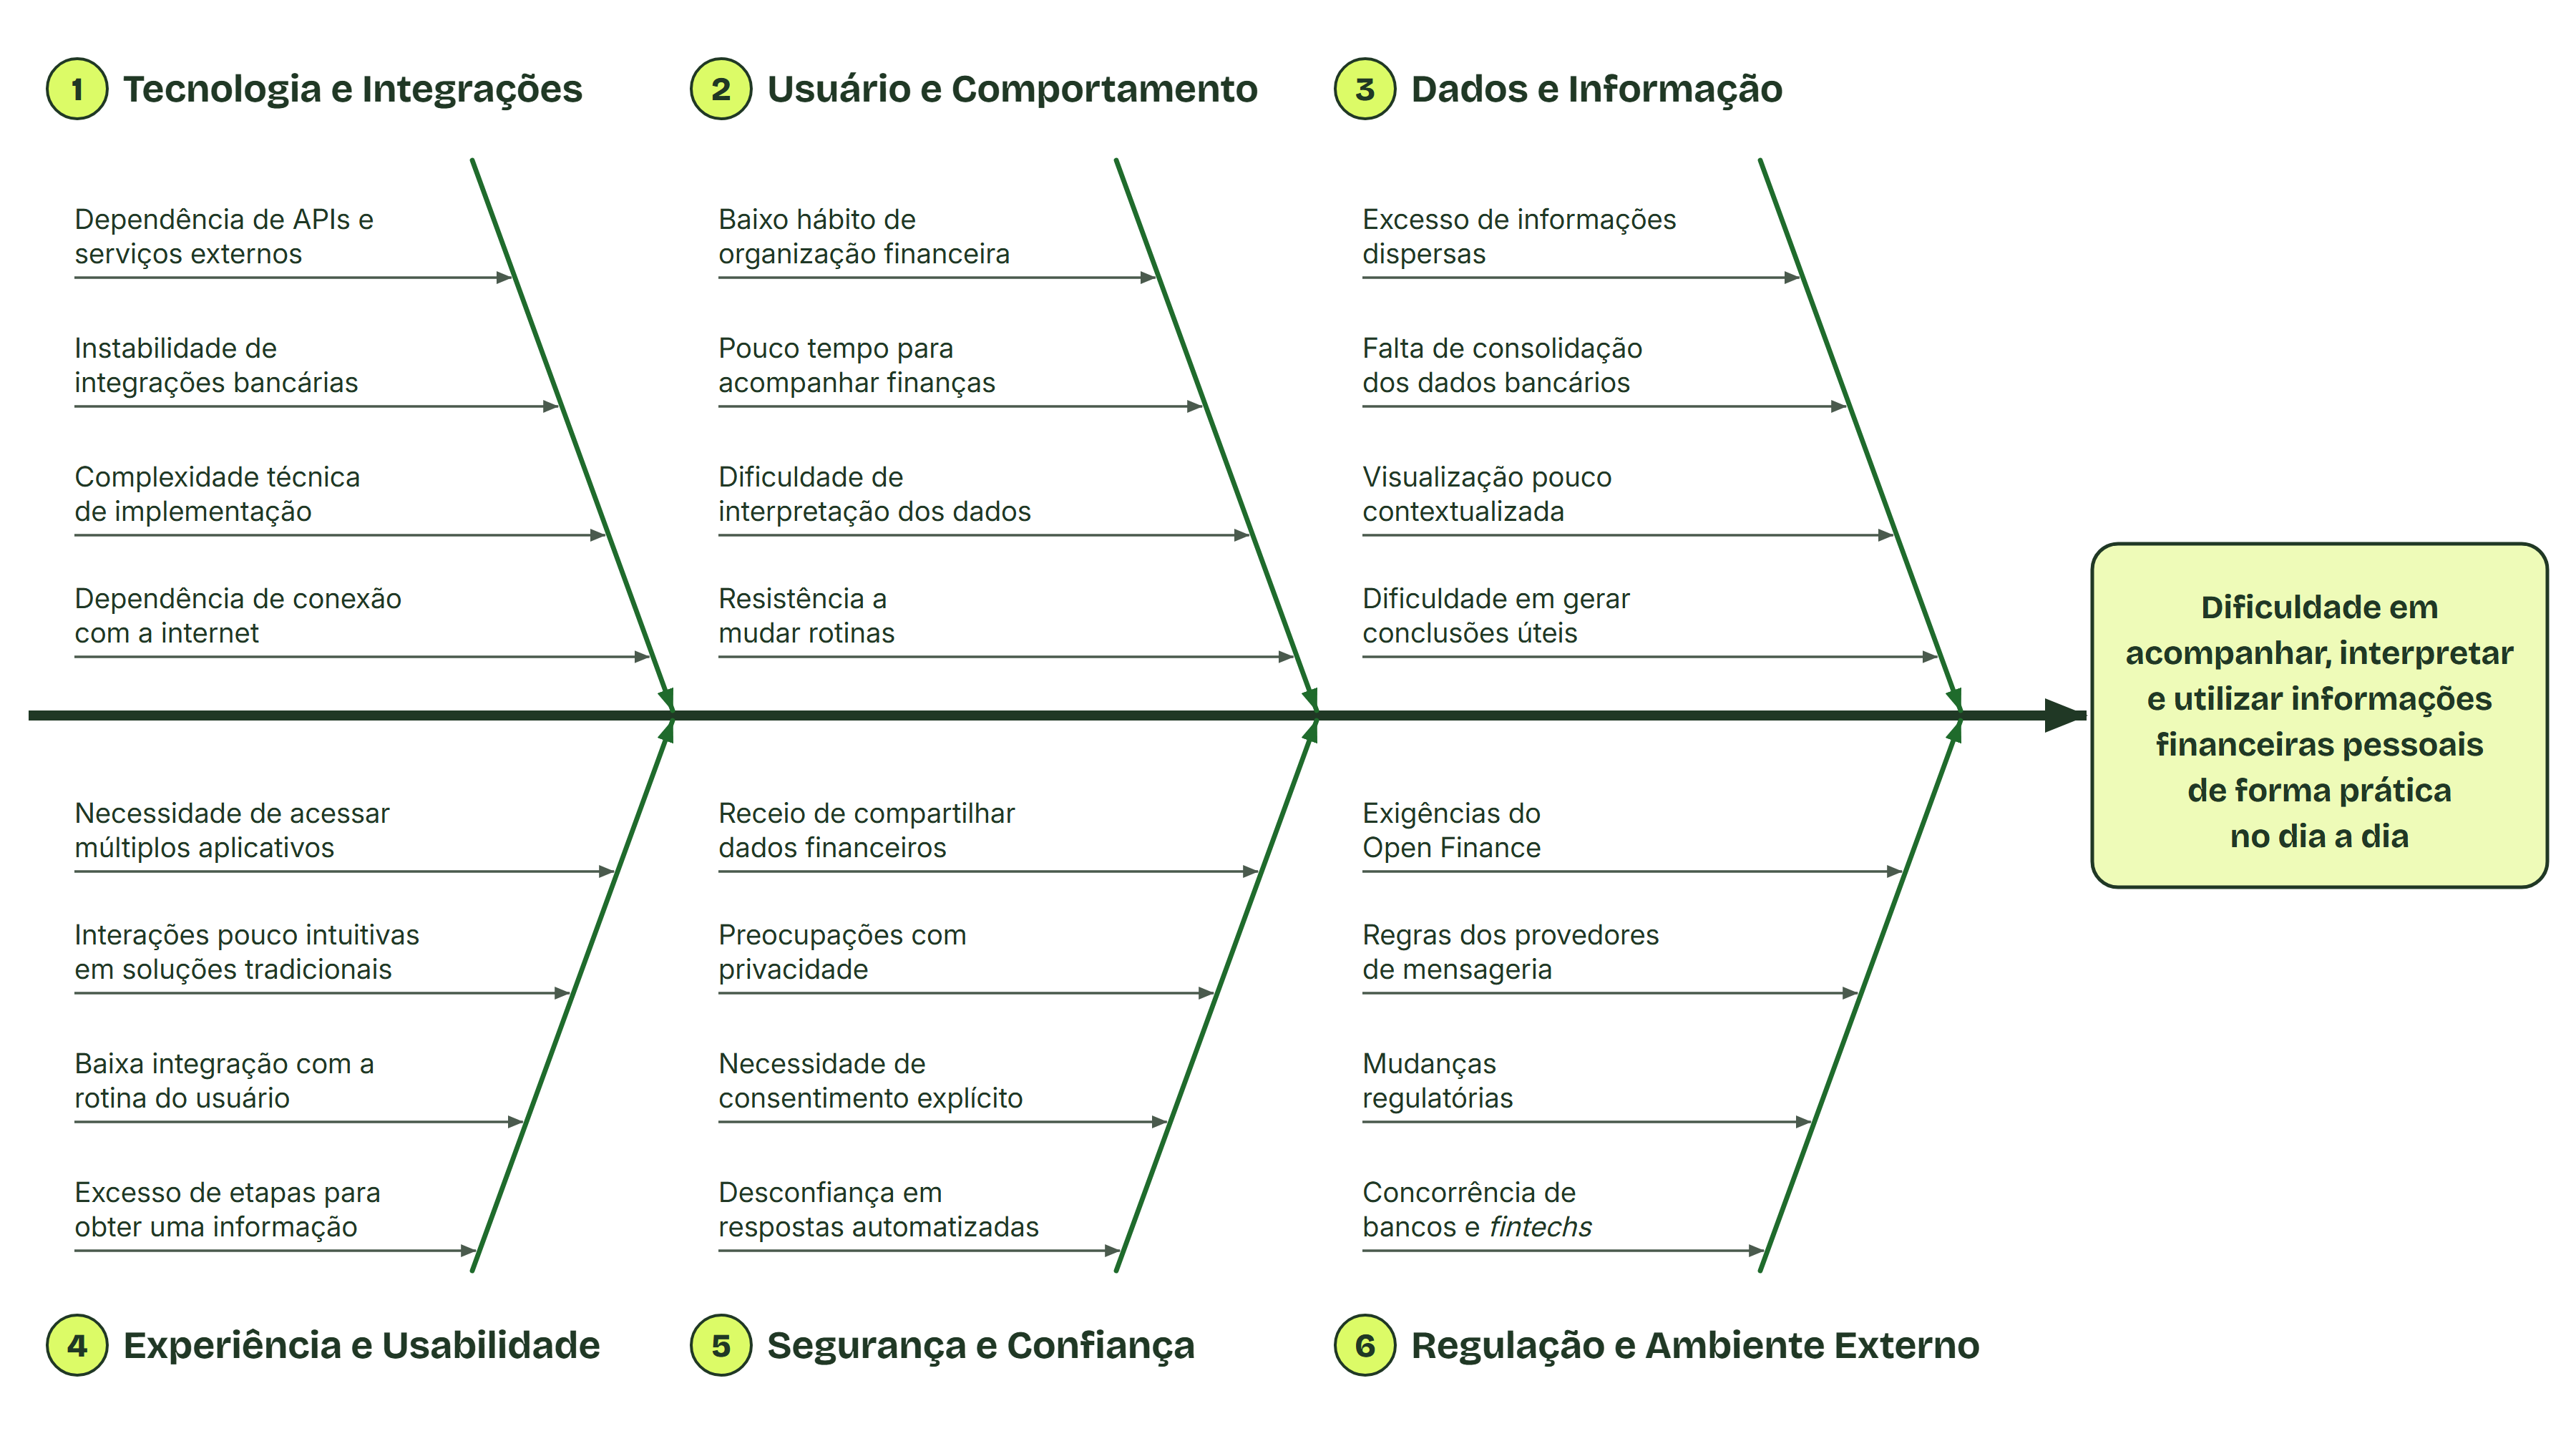
\includegraphics[width=1\textwidth]{images/ishikawa.png}
    \sourcenote{\textbf{Fonte:} Elaborado pelos autores (\workYear), com base em Ishikawa (1985).}
\end{figure}

O diagrama organiza as causas do problema em seis categorias. As de tecnologia e integrações e as de dados e informação mostram a dispersão dos dados entre instituições e a dificuldade de transformá-los em conclusões úteis, o que orientou a integração com o Open Finance e o cálculo dos valores sobre dados estruturados. As de usuário e comportamento e as de experiência e usabilidade mostram que o acompanhamento depende da iniciativa do usuário e do acesso a vários aplicativos, o que levou a conversa para o mensageiro que ele já usa e motivou os avisos e resumos proativos. As de segurança e confiança e as de regulação e ambiente externo explicam a atenção dada ao mascaramento por PIN, ao consentimento explícito e à independência em relação aos provedores de mensageria. Essas causas servem de base para os requisitos apresentados no capítulo seguinte.
